\setcounter{step}{0}

\subsection{ Buchty na pare }

\begin{ingredient}
  
      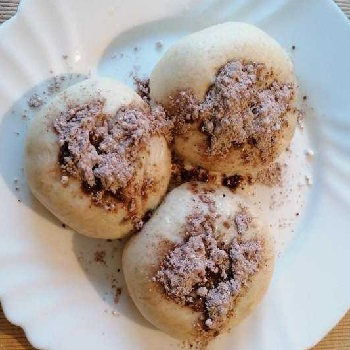
\includegraphics[height=5.5cm]{images/buchty_na_pare}
  
  \def\portions{  }
  \textbf{ {\normalsize Ingrediencie (4 porcie):} }

  \begin{main}
      \item 700g polohrubá múka
      \item 1ks droždie
      \item 400ml mlieko
      \item 30g kryštálový cukor
      \item štipka soľ
      \item plnka (nutela, džem)
  \end{main}
  
\end{ingredient}
\begin{recipe}
\textbf{ {\normalsize Príprava:} }
\begin{enumerate}

  \item{Z teplého mlieka, droždia, cukru, kúsku múky a štipky soli urobíme kvások}
  \item{Vypracujeme hladké cesto, necháme 45 minút vykysnúť}
  \item{Vyvaľkáme na 1cm a urobíme buchty}
  \item{Paríme asi 10 minút}

\end{enumerate}
\end{recipe}

\begin{notes}
  
\end{notes}	
\clearpage
